\section{Methodology}

Steps: Pretraining(CE Loss), Training (loss on target only)

Context:
Dialog History like SimpleTOD
DST instead of dialog history

Additional info
Schema
List of system actions
User actions
Service Results

\begin{itemize}
    \item Summary and importance of approach
    \item Base model (GPT-2)
    \item Prompt (context, additional info)
    \item Training (pretraining, training)
\end{itemize}

\begin{figure*}
    \centering
    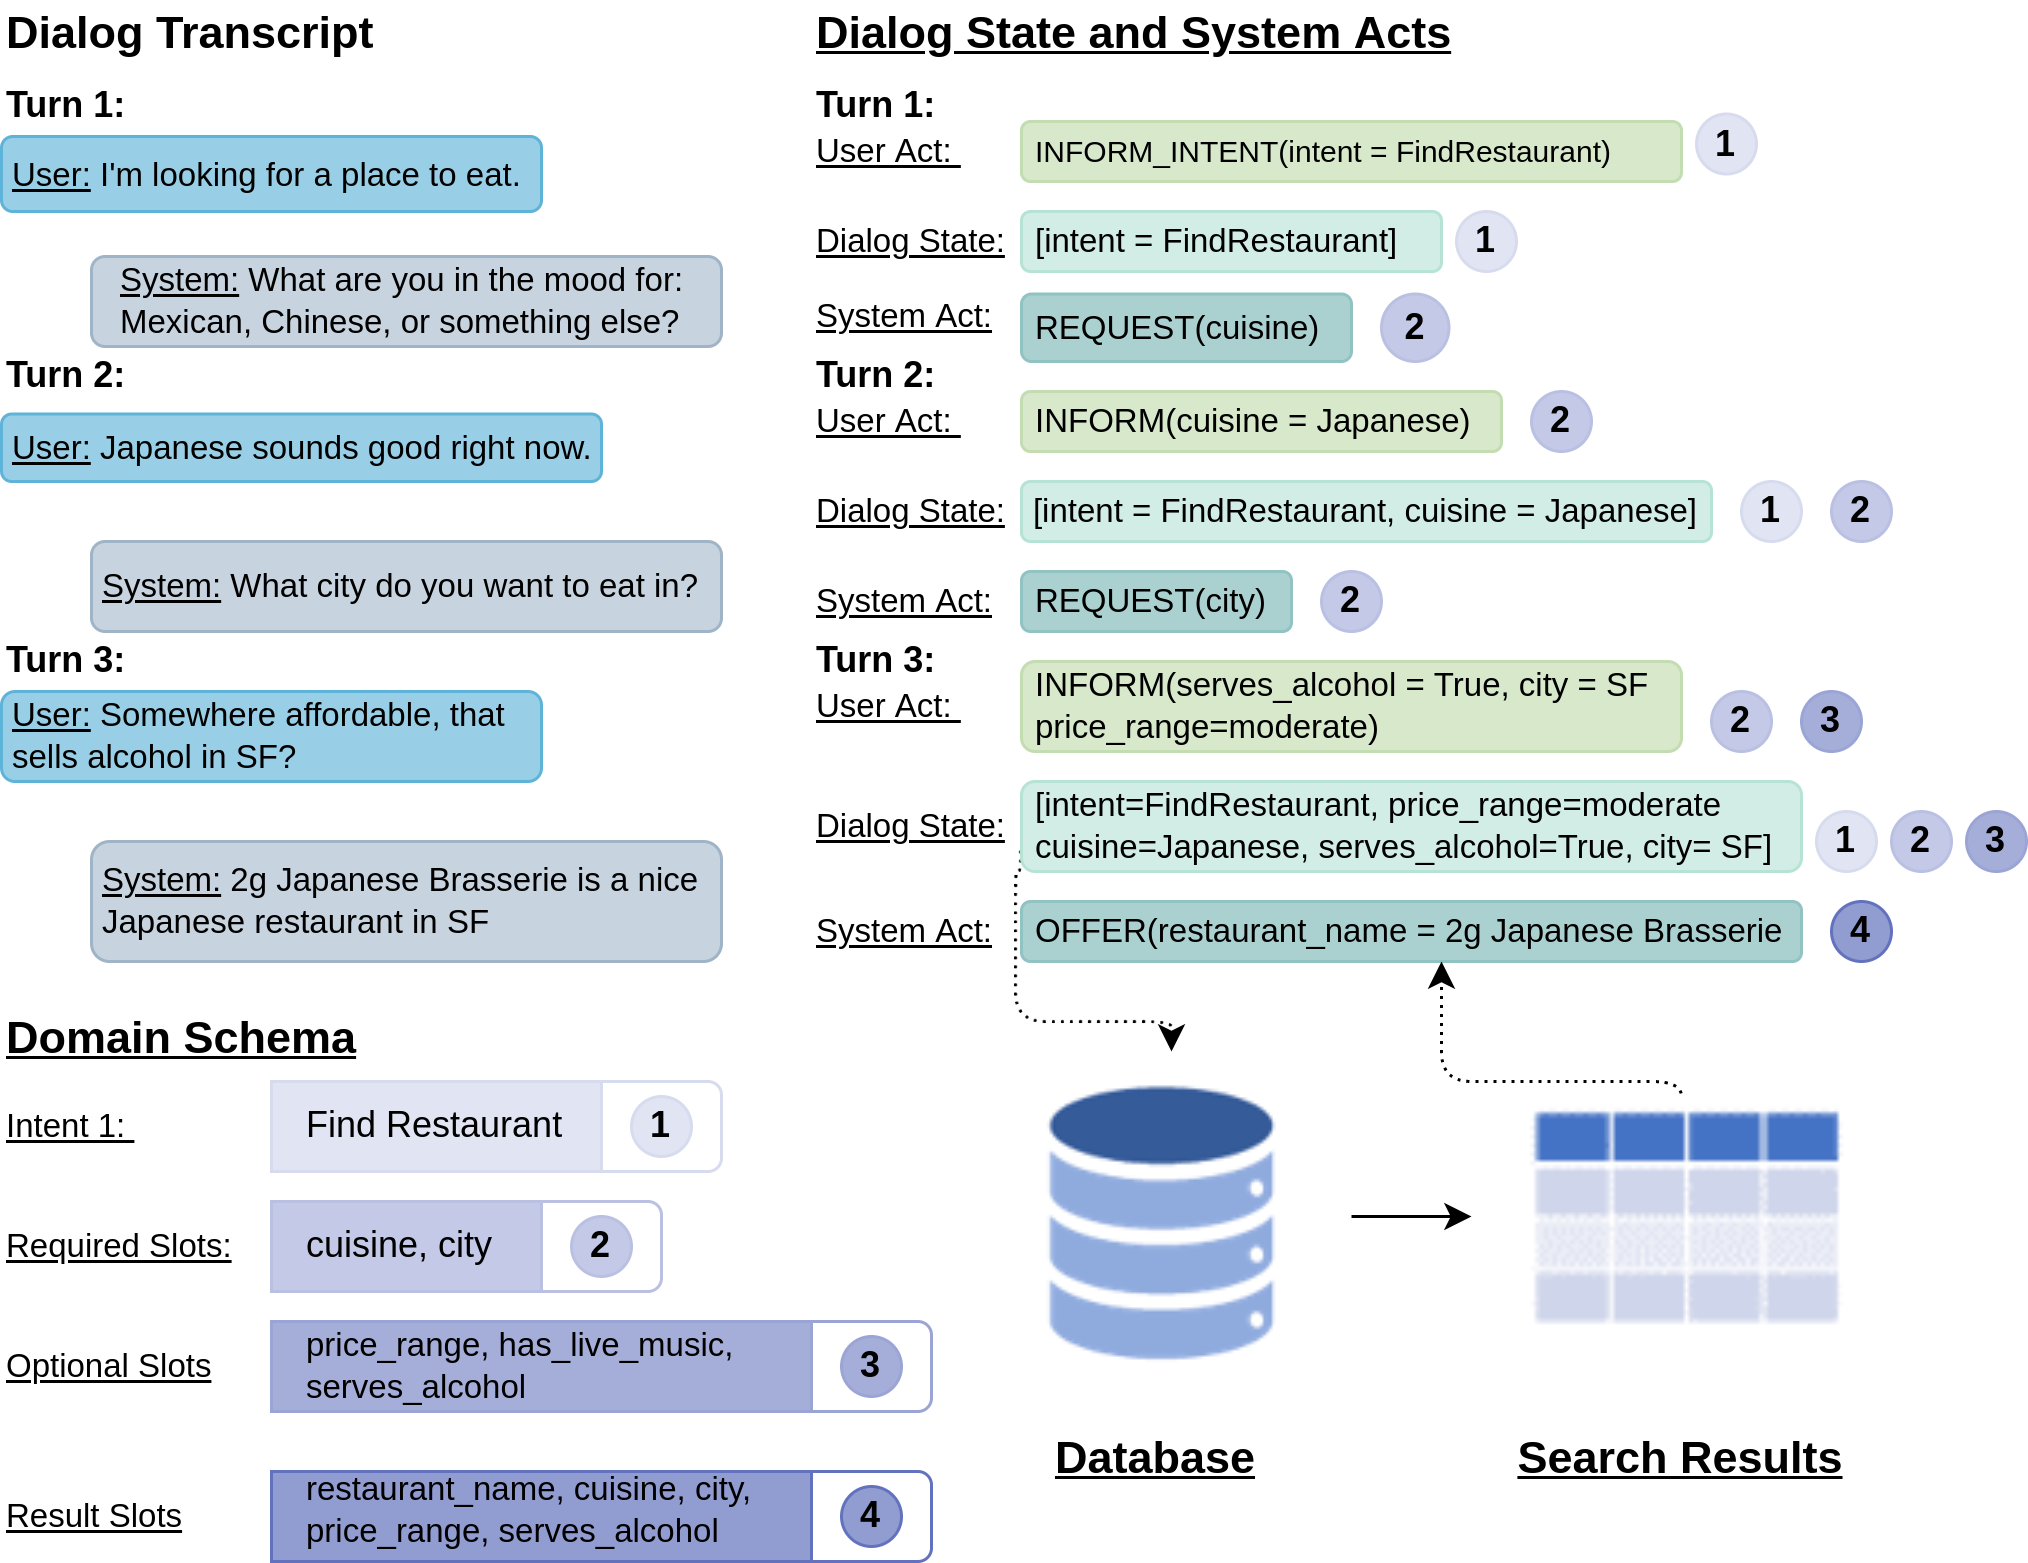
\includegraphics[width=\linewidth]{assets/approach.png}
    \caption{
        Using the user utterance (brown), domain schema (blue), system action names (purple) and database results, our model autoregressively generates the dialog state (green),
        user actions (yellow) system action (red) and system response (gray)
    }
    \label{fig:approach}
\end{figure*}

\subsection{Problem Formulation}

A dialog session is composed of multiple turns, which consists of interactions between the user and the system
in natural language utterance.
The SGD dataset provides a list of Schemas, $S = (s_1, ...., s_n)$ and each dialog contains a list of service names, which
can be used to extract the relevent schema for that dialog, $S_r \in S$.

For a turn $t$, the inputs to the model are the following: user utterance $U_t$, DST from the previous turn $D_{t-1}$, relevant schemas $S_r$, database search results $Db_t$
and a list of system action names $Action_{all}$.
The model autoregressively generates the dialog state $D_{t}$, user actions $UA_t$, system actions $SA_t$ and system response $R_t$.
Figure~\ref{fig:approach} shows a visual representation of the overall approach.


\subsection{Training}

The model is trained in two steps, where in the first step we calculate the cross entropy loss on the context and target,
and in the second step we calculate the loss only on the target.
The intuition behind this is that in the first step the model understand the general structure of the text
and in the second step the model fine tunes the target text.

